\documentclass{llncs}
\usepackage{graphicx}
\newcommand{\todo}[1]{\textbf{#1}}

\begin{document}
\title{TrueGrid: Code in a Grid and Grids in the IDE}
\author{Felienne Hermans \and Tijs van der Storm}
\institute{TODO\\
	\email{f.f.j.hermans@tudelft.nl}\\
	\email{todo}} 
\maketitle
\begin{abstract}
Spreadsheet systems are live programming environments. Both the data and the code are right in front you, and if you edit either of them, the effects are immediately visible. Unfortunately, spreadsheets lack mechanisms for abstraction, such as classes, function definitions etc. Programming languages excel at abstraction, but most mainstream languages or integrated development environments (IDEs) do not support the interactive, live feedback loop of spreadsheets. As a result, exploring and testing of code is cumbersome and indirect. 

In this paper we propose a method to bring both worlds closer together. We propose TrueGrid: an approach where spreadsheet cells can be programmed not with formulas but a full featured programming language (JavaScript).

We then describe TrueGrid within two different worlds: the spreadsheet world, where it adds the benefits of source code, including added abstractions, syntax highlighting, version control. We then describe TrueGrid within the IDE, where it brings the benefits of the liveness of spreadsheets which will support rapid application development.
\end{abstract}

\section{Introduction}
\subsection{Spreadsheets}
Spreadsheets are very popular tools for end-user programming \todo{cite proof}. Their formula language is easy to learn and their grid interface is inviting. Apart from this, spreadsheets have the interesting propoerty of being \emph{live} programming. First proposed as a design principle by Maloney and Smith \cite{maloney_directness_1995}, liveness indicates that a user interface is always active and reactive. According to \cite{maloney_directness_1995} in a live interface ``objects respond to user actions, animations run, layout happens, and information displays are updated continuously''. More recently live programming has found its way to the public eye, among others by Bret Victor in his talk `Inventing on Principle' \cite{Victor2012}. Figure \ref{fig:bret}, taken from Victor's talk, illustrates the idea of live programming: on the right, we have source code and on the left, we have the result of that code, in this case: a tree. Modifying the code will immediately affect the tree.
 
This liveness is one of the core features of most spreadsheet systems. When a users enters a formula and presses enter, they see the result, without any effort such as compilation. Liveness of spreadsheets powers a spreadsheet's flexibility, often praised as their key success factor.

\begin{figure}
  \begin{center}
  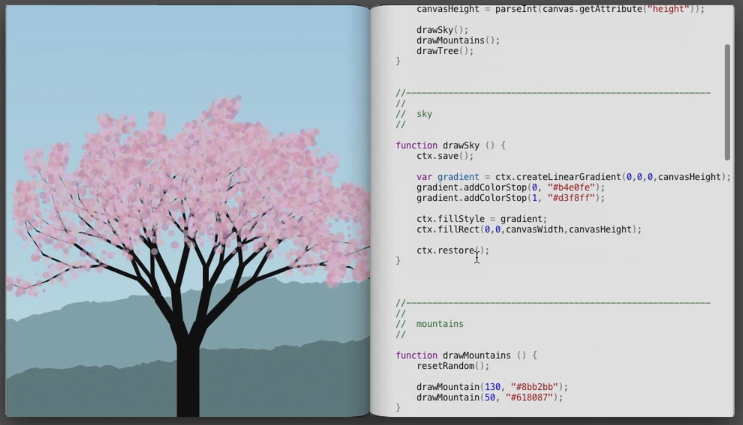
\includegraphics[width=9cm]{fig/bret.png}
  \caption{Live programming: on the right the source code and on the left its instantiation of the code which changes immediately when the code is updated, screenshot from~\cite{Victor2012}.}
  \label{fig:bret}
  \end{center}
\end{figure} 

However, spreadsheets have a number of downsides too, for example the lack of possibilities to abstraction. Instead of creating objects and methods on them, spreadsheet users mimic abstraction by copy-pasting formulas \todo{references naar LIVE paper}. Secondly, the editor that Excel and other spreadsheet systems provide is very limited, for example lacking syntax highlighting and not inviting proper structuring of formulas. 

\subsection{Code}
On the other hand, there is source code. Most existing programming languages do support abstraction, and modern editors help developers understand and structure their code. However, source code does not have liveness \todo{apart from a few recent initiative that have not been adopted mainstraim, Tijs, hedd gij dr paraat?} 

%\subsubsection{Directness}
%Another benefit of spreadsheets is that their interface combines data, metadata and calculations together in one view, and provides the user with easy access to all. Just by clicking a formula, one can manipulate it. This is often called `directness': \emph{``the feeling that one is directly manipulating the object''} \cite{shneiderman_direct_1983}. From a cognitive perspective, directness in computing means \emph{``a small distance between a goal and the actions required of the user to achieve the goal''} \cite{burnett_visual_2001}.

%Maloney and Smith describe directness as the fact that a user can \emph{``can initiate the process of examining or changing the attributes, structure, and behavior of user interface components by pointing at their graphical representations directly, as opposed to navigating through an alternate representation.''}\cite{maloney_directness_1995}.

%This almost exactly describes the interface of a spreadsheet. Instead of navigating to a code behind, a class or an object, spreadsheet users have all ingredients: data, metadata and calculations, in one view, and can access them with one click. 

\section{TrueGrid}
In this paper, we will describe an approach bridging the gap between programming and spreadsheets and describe ts implications in both worlds. The basic concept of TrueGrid is a grid which can be programmed in a fully featured programming language, where the grid and the code are juxtapositioned ed, like in a spreadsheet, as demonstrated in Figure \ref{fig:TG}. Furthermore, like a spreadsheet, TrueGrid is live, i.e. on a change of data or code, the grid is updated.

\begin{figure}
  \begin{center}
  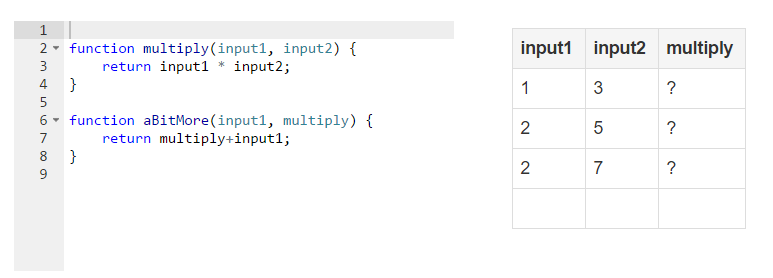
\includegraphics[width=9cm]{fig/TG.png}
  \caption{A True Grid \todo{make ss with syntax highlighting, and add explanation}}
  \label{fig:TG}
  \end{center}
\end{figure} 

In our example, we use JavaScript as a language, however, the idea itself is not limited to one programming language, in fact, one can even image a grid in which different programming languages live.

\section{TrueGrid for Spreadsheet Users}
As an implementation of TrueGrid for spredsheet users, we hypothesize that it will be embedded within an existing spreadsheet system, allowing users to use advanced features like PivotTables and charts on top of their TrueGrid. For spreadsheet users, using TrueGrid over spreadsheets presents several benefits. For example, a programming language enables the use of modern editors. In the above example we have used Ace \todo{add link} providing syntax highlighting and syntax errors for free. Furthermore, the textual form of the code allows for easy diffing, merging enabling more mature version control on grids. While learning a new programming language can be challenging, there are spreadsheet developers working with VBA now, which is a fully featured language, and we envision TrueGrid having a lower threshold as the liveness and juxtaposition will ease understanding.

\section{TrueGrid for Developers}
Like spreadsheet users, developers often work with (example) data when programming. In modern IDEs, it is not possible to load data and then program alongside it. This makes it difficult for quickly prototype simple data analysis projects. A TrueGrid embedded in the IDE


Using TrueGrid, a programmer you can inspect data and play with an initial implementation, before having to write interfaces or even unit tests. We envision this is a useful tool very early in the development process, when you have some data and only a vague idea of where the project is going. 

For example, consider the situation where a developer has a list of number that you want to manipulate \todo{We need a better example here} Before she even wants to write tests, the developer might want to explore the dataset a bit, for example, by sorting, calculating the mean or outliers. These type of activities currently have to be done outside of the IDE, for example in Excel or using a scripting language like R. Using TrueGrid this activity can be performed within the IDE.


\section{Related Work}
\todo{tsja}

\bibliographystyle{splncs03}
\bibliography{references}
\end{document}